\documentclass{article}
\usepackage[utf8]{inputenc}

% Tables
% Use Roman numerals for tables
% https://tex.stackexchange.com/a/226029
\usepackage[labelsep=period]{caption}
\captionsetup[table]{name=Table}
\renewcommand{\thetable}{\Roman{table}}
% \usepackage{multirow}

\usepackage{pdflscape}
\usepackage{gensymb}

\usepackage{subcaption} % For subfigures?

% units
% \SI{X}{\UNIT} will write the value X with units \UNIT. 
% eg. \SI{30}{\celsius}
\usepackage{siunitx} 

\usepackage{graphicx}
\graphicspath{ {./images/} }

\usepackage{todonotes}
\newcommand{\tino}[1]{\todo[inline,color=purple!40]{Tino: #1}}
\newcommand{\fbp}[1]{\todo[inline,color=orange!40]{Ferran: #1}}
\newcommand{\summary}[1]{\todo[inline,caption={},color=yellow!40]{Summary: \\ #1}}

\newcommand{\ssr}[1]{{\textbf{\textcolor{blue}{Shashank: #1}}}}

\newcommand{\gbox}[1]{{
\fbox{
\parbox{0.8\textwidth}{  \fbox{$\triangleright$\textcolor{blue}{\textbf{Gon}:}} 
#1
}}}}

\usepackage[normalem]{ulem}

\setlength{\textheight}{8.4in}
\setlength{\topmargin}{0.1in}
\setlength{\headheight}{0.2in}
\setlength{\headsep}{0.1in}
\setlength{\oddsidemargin}{0in}
\setlength{\textwidth}{6.5in}

\title{Knees in lithium-ion battery lifetime}
\author{To do}
\date{}

\begin{document}
\maketitle

**PREVIOUS DRAFT IS NOW IN main\_old\_experiment\_then\_model.tex**

\section{Introduction}

Lithium-ion batteries will continue to play a critical role in decarbonization via their use in electric vehicle and stationary energy storage applications. One of the most challenging requirements for these demanding use cases is long lifetime, with typical warranties of X years for electric vehicles and X years for grid storage[lit values?]. Battery lifetime requirements will only become more demanding as “million-mile batteries” become the expectation for next-generation electric vehicles. Furthermore, as concerns around battery mining, manufacturing, and disposal increase, improving battery lifetime is a straightforward way to reduce the environmental impact of the lithium-ion battery lifecycle. Thus, understanding and improving the lifetime of lithium-ion batteries is a critical research direction.

Lithium ion batteries often exhibit one of three degradation patterns: linear, sublinear, or superlinear aging (Figure 1). In laboratory settings (i.e., single-cell testing using battery cyclers), degradation is typically presented as capacity or energy vs. cycle number. Cells often degrade linearly[] or sublinearly[]. Sublinear degradation is often attributed to side reactions such as the solid-electrolyte interphase (SEI) growth, which grows approximately[] (but not exactly[]) with the square root of time or cycle number due to its self-passivsting nature. While this type of degradation is largely unavoidable, the decelerating degradation rate is a fortunate property for long-lifetime applications. However, superlinear battery degradation is also often observed (Figure 1c). This type of degradation goes by many names in the battery literature, including “knee”, “rollover failure”, “sudden death”, “accelerated aging”, “nonlinear aging”, etc; we use the term “knee” in the remainder of this work. Avoiding this type of degradation is critical to ensure long lifetimes in the field. However, despite many experimental and modeling reports on this topic, a comprehensive understanding of knees is lacking, likely due to the variety and complexity of proposed mechanisms.

{
\centering
\includegraphics[scale=1]{figures/degradation_rates.eps}
}

In this review, we survey the literature and critically examine both experimental and modeling work on the subject of knees. We first review methods to define the knee point. We then classify experimental observations of knees in the literature; broadly, all cells with differences in knee behavior can be attributed to either differences in design, differences in usage conditions, or cell-to-cell/testing variation. Finally, we briefly discuss physics-driven and data-driven approaches to knee prediction, practical guidelines for avoiding knees, and suggested future work on this topic. This review can serve both academic and industrial efforts to understand and improve battery lifetime.

\section{Defining the knee point}

Locating a knee is easy by eye for a single, smooth and ideal health profile (e.g.\ around 400 cycles in figure 1). However this becomes trickier in cases where one has many cells with distinct lineshapes caused by intrinsic and extrinsic variability. Noise and erroneous data collection can also cause issues with identifying a knee.

{
\centering
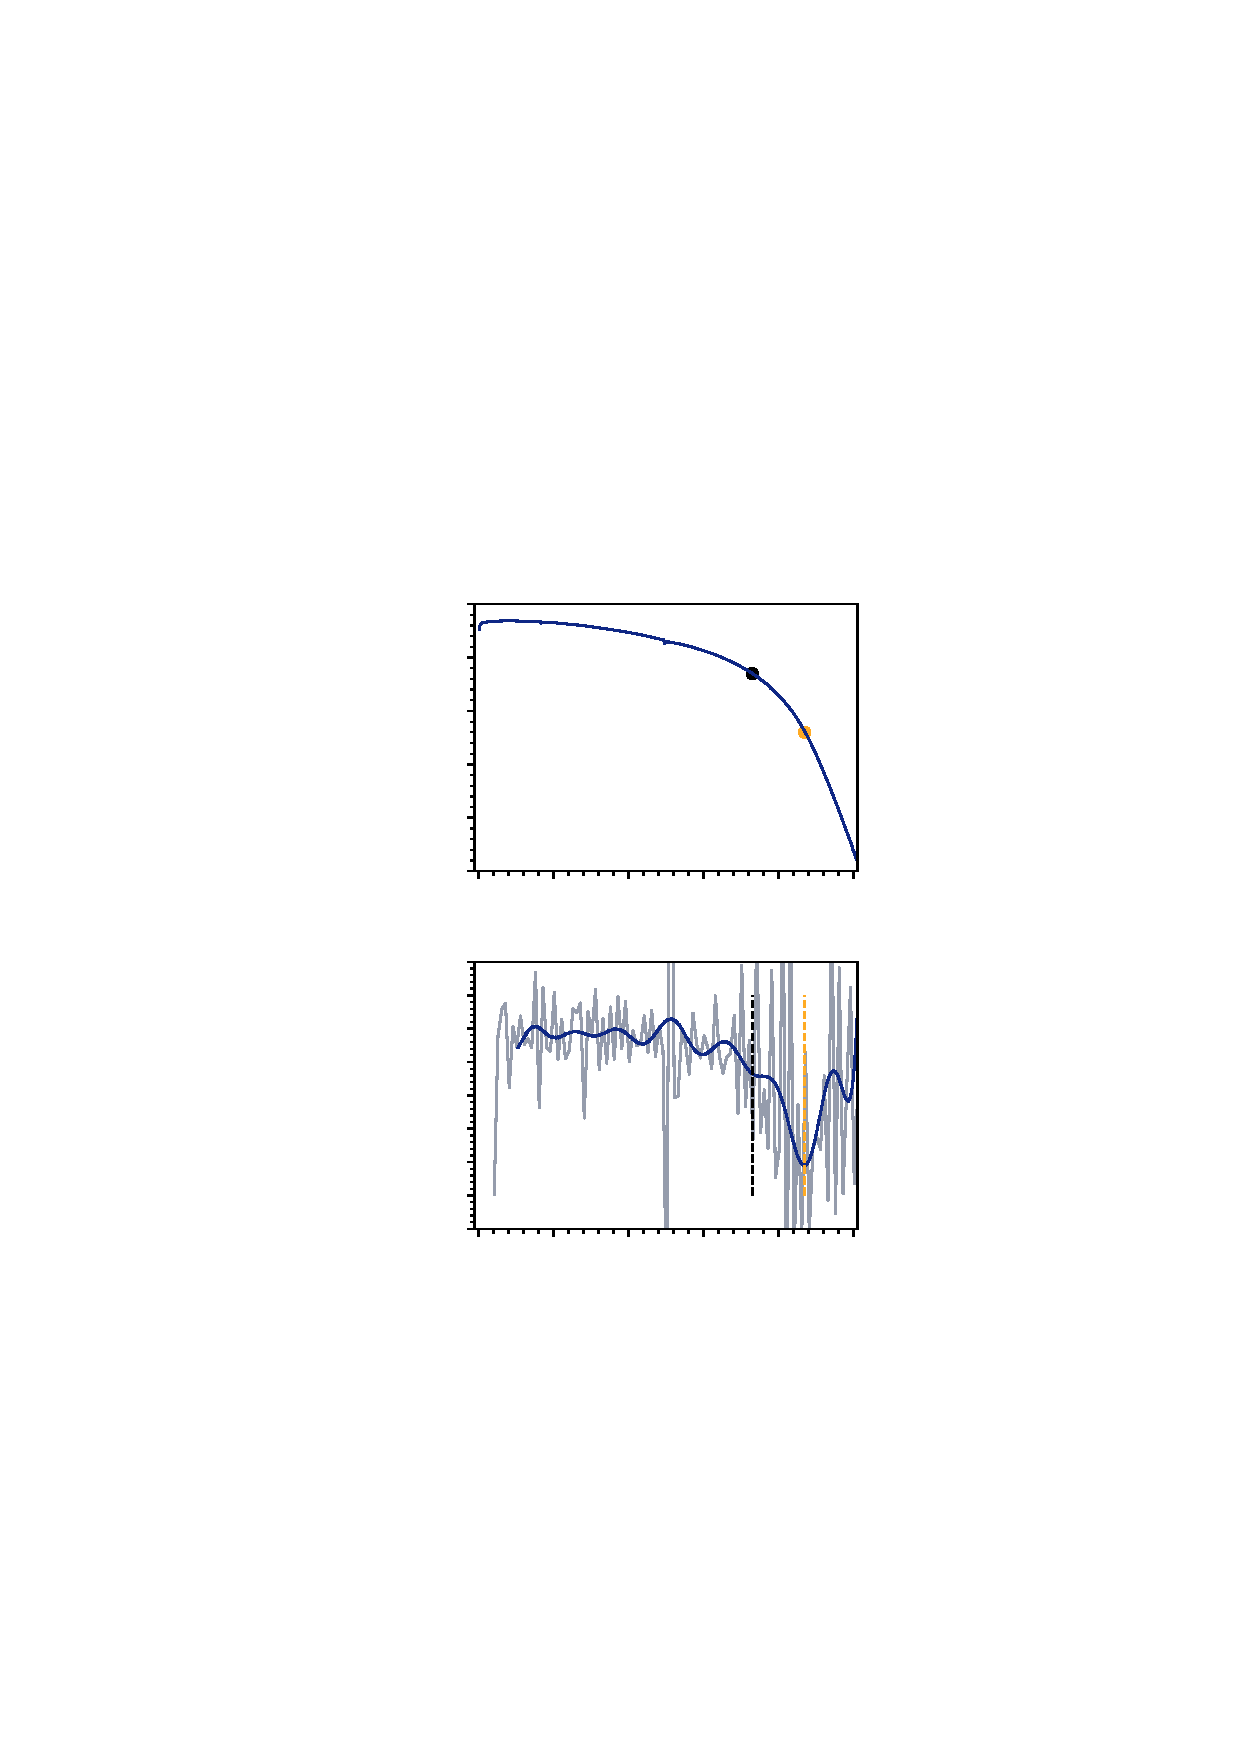
\includegraphics[width=\textwidth]{images/knee_definition.pdf}
\label{fig:knee_definition}
}

Mathematically, the knee would be described as the point at which degradation rate is changing fastest, i.e.\ the second derivative reaches some maximal value. However that point appeared slightly after where we put the knee, and figure 2 demonstrated how even very small amounts of noise ($\sigma=0.05\%$ capacity) cause significant issues. Consequently, we concluded that health metric profiles should be smoothed prior to knee identification.

Several knee point identification methods have been applied in literature. Figure 2 includes an identification mechanism that is more robust to noise.

Figure 2. Bacon-Watts, etc




\begin{figure}[ht]
\centering
\begin{subfigure}{.5\textwidth}
  \centering
\includegraphics[width=1.1\linewidth]{figures/AcrossDatasetsknee-to-EOL}
  \caption{Linear regression of knee-point to EOL point}
  \label{fig:kneepoint2EOL}
\end{subfigure}%
\begin{subfigure}{.5\textwidth}
  \centering
%   0.50\textwidth
  \includegraphics[width=1.1\linewidth]{figures/AcrossDatasetsonset-to-knee}
  \caption{Linear regression of knee-onset to knee-}
 \label{fig:kneeonset2kneepoint}
\end{subfigure}
\caption{Total of 306 cells across 15 datasets. (a) Linear relation between knee-point and EOL while (b) Linear relation between knee-onset and knee-point.}
\label{fig:knees2EOL}
\end{figure}









\gbox{
Plan for the section (identify the references):
\begin{itemize}
    \item discuss definition (point to IEE standard; point that def is qualitative)
    \item Very brief Overview of methods (BW, Kneedle, Diao, Bissector, quantile). Wrap with small Table with notes
    
    include qualitative comparison of methods (via linear regression to EOL)
    \item Present empirical analysis plot of linear regressions across datasets for knee-2-EoL
    \end{itemize}
}



%%%%%%%%%%%%%%%%%%%%%%%%%%%%%%%%%%%%%%%%%%%%%%%%%%%%
%%%%%%%%%%%%%%%%%%%%%%%%%%%%%%%%%%%%%%%%%%%%%%%%%%%%
%%%%%%%%%%%%%%%%%%%%%%%%%%%%%%%%%%%%%%%%%%%%%%%%%%%%
%%%%%%%%%%%%%%%%%%%%%%%%%%%%%%%%%%%%%%%%%%%%%%%%%%%%
\section{Pathways for knee points}

Figure 3. 
{
\centering
\includegraphics[scale=1]{figures/snowball_vs_hidden_mechanism.eps}
}

Also include schematic on all pathways
\subsection{Litihum Plating}
\subsubsection{Direct Thermodynamic Lithium Plating}
Li inventory loss due to thermodynamic Li plating may occur whenever there is not enough negative electrode capacity to store all of the available lithium during charging.  This well-known plating mode has been used intentionally by several researchers.  Martin et al [1] used deposited Li metal as a mechanism to store extra capacity, enabling the cell to occasionally discharge extra energy without requiring a larger anode,effectively increasing the specific volumetric energy density of the cell.  Researchers at Sandia National Lab also created cells with limited negative electrode capacity (N:P ratios of 0.75 and 0.5) to intentionally deposit Li metal to study the failure behavior of cells after Li plating has occurred [2].
\subsubsection{Direct Kinetic Lithium Plating}
Li plating may also occur heterogeneously, when the local Li+ potential exceeds the nucleation barrier, leading to direct plating even in cases where the average graphite to Li potential would not lead to plating. Direct heterogeneous Li plating can be driven by a wide range of design and usage conditions; the prototypical usage case leading to Li plating is high charging rates at low temperature \cite{waldmann_temperature_2014, petzl_lithium_2015}. Waldmann et al showed utilization of Arrhenius plot for ageing mechanisms at lower temperature ranges (below \SI{25}{\celsius}). At low temperatures, lithium ions have less energy to cross the potential barrier on SEI and in graphite electrodes. This low temperature plating was validated by experiments on 18650 pouch cells of LNMC and LMO blends and graphite anode. Note that there are no consistent quantitative values for ‘high’ charging rate or ‘low’ temperature, as plating will occur whenever the local potential exceeds the energy barrier for Li nucleation. Thus, plating may be observed even at fairly normal test conditions, such as 1C CC charging near room temperature \cite{waldmann_optimization_2015,burns_-situ_2015}. Increasing temperature and cell design may allow for much more rapid charging before Li plating and knee-over is observed; Lewerenz et al cycled cells at rates up to 8C, observing no obvious knee-over up to 4C, though microstructural evidence of Li plating was found even at 1C \cite{lewerenz_systematic_2017}. The onset of direct lithium plating is also very sensitive to the charging protocol, with many studies demonstrating that informed design of charge protocols can substantially extend cell lifetime by preventing direct lithium plating \cite{waldmann_optimization_2015,schindler_fast_2018}.
Mechanical stress on the cell pouch or cell casing may also lead to direct kinetic lithium plating, as applied stress can compress the electrode. This reduces the porosity of the electrodes in a small region, reducing the diffusivity of electrolyte and thus increasing the local polarization and potentially causing lithium plating. A direct test of this cause was conducted by Liu and Arnold \cite{liu_effects_2020}, who demonstrated that localized lithium plating could be controlled by densifying regions of the separator, which decreases the local lithium diffusivity and led to localized lithium plating. Many examples exist mechanical stress leading to lithium plating, as well. For example, Bach et al applied a hose clamp around the circumference of an 18650 cell, and a post-test tear down clearly showed lithium plating localized to regions of the electrodes that were under compressive stress \cite{bach_nonlinear_2016}. Pouch format cells also show similar results. Fuchs et al \cite{fuchs_post-mortem_2019} applied pressure using a metal bearing. Liu et applied pressure to electrodes in a coin cell setup using various shapes, producing legible shapes and letters using localized lithium plating \cite{liu_size_2018}.
(copied from 'Mechanical degradation section, remove either section)

Design conditions - anode porosity, electrode channels, particle sizes / distribution….? Experimental evidence? Lots of modeling work on micro-structure being done at NREL.

\textbf{Mechanically induced heterogeneous lithium plating - Phillip and Tino analysis of empirical results}

\subsubsection{$\textbf{LAM}_{deNE}$}
( Surface layer growth, Delamination, Dry Out):
Loss of active material of NE for lithium insertion is caused mainly due to particle cracking and electrical contact loss/blockage of active sites by resistive surfaces. Lithium trapped inside isolated graphite particles can contribute to cell capacity decrease due to unavailability to cycle. 

K.Jalkanen et al \cite{jalkanen_cycle_2015} showcased cyclic aging at different cycling temperatures (\SI{25}{\celsius}, \SI{45}{\celsius} charge and \SI{65}{\celsius} discharge) through capacity fade. At temperatures above \SI{60}{\celsius}, aging at NE (graphite electrodes) is different compared to low temperature aging. Elevated temperatures contribute to excess Li plating during  cycling apart from the SEI-layer increase on anode surface which occurs during normal charging and discharging cycles at room temperature. Increase in SEI-layer thickness enhances graphite electrode polarization leading to additional plating. SEI-growth also leads to electrolyte consumption due to prolonged cycling at high temperatures. Irreversible lithium plating reduces graphite electrical contact, when lost, results in isolated dead lithium and capacity degradation \cite{petzl_lithium_2015}.  

THIS NEEDS REWORKING AND FOCUSING

Jalkanen et al. found significant Li plating resulted from cycling at high temperature - 1 C charge/discharge at \SI{45/65}{\celsius} respectively \cite{jalkanen_cycle_2015}. 

Electrode sites may become inaccessible due to electrolyte dry-out. Electrolyte dry-out occurs in electrolyte lean cells due to decomposition of the electrolyte into gas and eventual de-wetting, causing some of the electrode to become inaccessible; cell gassing and dry-out often occurs in parallel with other degradation modes, and is thus difficult to deconvolute from other degradation modes during cycle aging. However, several calendar aging experiments have been conducted to investigate gassing and electrolyte dry-out impacts on cell performance. Mao et al clearly demonstrated the impact of dry-out during calendar aging at high temperatures, connecting accelerated capacity fade to gassing and electrolyte dry-out \cite{mao_calendar_2017}. They also determined that a small stack pressure of about 4 PSI mitigates the occurrence of dry-out within the porous electrodes due to gas formation by displacing gasses to the edges of the cell pouch. Xiong et al studied the impact of storage potential, temperature, and electrolyte composition on the volume and composition of gasses generated by electrolyte decomposition, finding that not only does electrolyte composition play a major role, but also that interactions between species generated separately at the anode and cathode is responsible for the decomposition of the electrolyte \cite{xiong_studies_2017}.
The impact of gassing and dry-out has been modeled by Kupper et al \cite{kupper_end--life_2018}.

Surface layer growth ...
Delamination ...
Dry out...

Localized loss of negative electrode active material sites can cause heterogeneous Li plating by impeding the transport of Li, locally increasing the over-potential and eventually causing plating. There are several mechanisms that may lead to LAMdeNE: surface layer growth, delamination, and electrolyte dry-out.

Surface layer growth on the negative electrode may impede Li transport into the negative electrode during charging. This surface layer has been often observed during accelerated aging of LIBs, and is most commonly attributed to Mn or Fe dissolution from the cathode and electrolyte salt decomposition \cite{lewerenz_post-mortem_2017,lewerenz_systematic_2017,zhu_investigation_2021,stiaszny_electrochemical_2014,rahe_nanoscale_2019,keil_linear_2019,sarasketa-zabala_understanding_2015, willenberg_high-precision_2020}. Lewerenz et al documented surface layer growth very thoroughly, finding that increasing C-rate and larger depth-of-discharge could lead to earlier onset of a knee, which was correlated with the presence of a thick surface layer on cells that contained knees; cells without knees also contained obvious surface layers, but with lower surface coverage and less thickness \cite{lewerenz_post-mortem_2017,lewerenz_systematic_2017}. These surface layers sometimes seem to lead directly to localized lithium plating, with lithium observed on top of the layer \cite{zhu_investigation_2021}.

Delamination may also lead to inaccessible negative electrode material, which can potentially cause lithium plating and knee-onset. Willenberg et al conclusively observed delamination induced knee-onset in cylindrical cells; delamination was caused due to mechanical stresses and deformation after the formation of a surface layer on the negative electrode \cite{willenberg_high-precision_2020}. Cannarella et. al. also observed surface layer growth and delamination as a function of stack pressure in multi-layer pouch cells \cite{cannarella_stress_2014}. Pfrang et al observed delamination in cylindrical cells, though sometimes without observing knee-onset \cite{pfrang_long-term_2018}.

\subsubsection{Pore clogging}
As SEI forms, it precipitates mainly in the pores of the anode, causing reductions in the volume fraction of the electrolyte in the anode (Sikha, 2004). The decreased volume fraction causes increased over-potential, ultimately leading to increased plating. The plating also helps to reduce the volume fraction, thus creating a positive feedback loop which accelerates aging(cite Yang 2017). This phenomenon also causes a voltage undershoot, particularly noticeable at high discharge rates (3C) (cite Yang 2017). Several authors have noted that a critical porosity exists around 0.05, and pore clogging beyond that induces the period of accelerated aging (cite Yang 2017, Muller, 2019). Additionally, some authors model the same effect by changing the diffusion coefficient as a function of cycle number (Keil, 2020). One possible mitigation for this issue is to use a graded or stepped porosity profile. Since most pore clogging occurs near the separator, having a higher porosity near the separator and a lower porosity near the current collector helps to slow the onset of the accelerated aging caused by pore clogging (Muller, 2019).
\subsubsection{Others}
Apart from the main mechanisms causing knees due to plating, few other causes are based on substantial and mild temporally thermal transient conditions lead to a rapid capacity fade in cells when compared with cells at a fixed equilibrium temperature. Temporal transient thermal gradients (40 \degree C to 0 \degree C) contribute to Li ions being plated as Li instead of intercalating, which accelerates capacity fade over subsequent cycles causing knees and ultimately resulting in jellyroll collapse. Equilibrium cells at 40 \degree C, 20 \degree C, 0\degree C and transient cells (40\degree C to 0 \degree C and 10 \degree C to 0 \degree C) are tested for understanding of the thermo-electrochemical coupling across different temperature (Carter 2019).Differential voltage from charging gives route to plating detection and discharging cycle showcases the degradation modes. Equilibrium cells at 40 \degree C and 20 \degree C show minimal degradation while equilibrium cell at 0 \degree C has initial minimal degradation, then a gradual decay midway. On the contrary, transient 10 \degree C to 0 \degree C cell and 40 \degree C to 0 \degree C cell show degradation at earlier cycles (8 and 5 respectively) (Carta, 2019). Transient 40 \degree C to 0 \degree C cell demonstrates high lithium stripping during initial discharge cycles due to thermal transient induced plating causing increase in anode thickness, pressure buildup in jelly role and capacity loss. The decrease in differential voltage for transient cells immediately with the start of the cycle shows the degradation evidence by lithium plating.  

there are other causes for lithium plating leading to knees such as \textbf{temporally transient thermal conditions}, with examples where the cell temperature changing from 40\degree C to 0\degree C %$\circC$ (GdR: I replaced "\circC" by "\degree C"; easy to undo if needed)
leads to a rapid loss in capacity compared to cells at a fixed equilibrium temperature. Studies have shown that over half the Li ions transferred in first charge is deposited as plated Li during thermal transients. The repeated plating and stripping of lithium is shown to cause rapid jelly roll collapse in cylindrical cells leading to capacity knees.

https://doi.org/10.3389/fenrg.2019.00144


\subsection{DCR growth}
Summary: DCR resistance affects when you hit your cutoff voltage during charging and discharging. DCR resistance itself is a function both of cell state-of-health as well as cell temperature. Increased DCR resistance will then also lead to increased heat generation during the flow of current, which can lower resistance as more current is passed over the cell; this may lead to different results depending on cell architecture (coin, cylinder, pouch, prismatic) and cooling. And of course, you can test at different cutoff voltages.

Increasing DC resistance during cycling may also lead to the onset of not only a knee in cell power but also in the accessible capacity. This is intuitive at high currents, when the cell may hit a voltage limit before the majority of lithium has been shuttled across the separator, leading to a lower measured capacity. However, during aging, this rate limitation may occur at much lower than expected C-rates, and appear as a knee in the plots of power and capacity versus cycles. This behavior was thoroughly studied by Ma et al \cite{ma_editors_2019} using lab-made 230mAh NMC532/graphite pouch cells, varying electrolyte composition as well as the type of graphite. Careful study using impedance measurements, both of the full cells as well as symmetric coin cells of the positive and negative electrodes, was used to isolate the loss of performance to a dramatic increase of the cathode impedance during aging. This DC resistance growth was attributed to electrolyte oxidation at the positive electrode, which varied according to the upper cutoff potential as well as the electrolyte composition. Similar onset of a capacity knee due to the selection of the electrolyte composition was previously observed by Li et al as well (Li et al 2018 Methyl acetate.. In Zotero but not here). This behavior has been documented in earlier studies as well, for instance, a detailed aging study by Ecker et al \cite{ecker_calendar_2014} observed knee onset correlated with dramatically increased DC resistance (200-400 percent).

DCR resources:
\begin{itemize}
    \item \cite{willenberg_high-precision_2020}
    \item \cite{broussely_main_2005}
    \item \cite{ecker_calendar_2014}***
    \item \cite{schuster_nonlinear_2015}
    \item \cite{lewerenz_systematic_2017}
    \item \cite{lewerenz_post-mortem_2017}
    \item \cite{martinez-laserna_technical_2018}
    \item \cite{ma_editors_2019}***
    \item \cite{braco_experimental_2020}
    \item \cite{frisco_understanding_2016}
    \item \cite{klett_non-uniform_2014}
    \item \cite{pfrang_long-term_2018}
    \item \cite{keil_linear_2019}
    \item \cite{keil_charging_2016}
    \item \cite{rahe_nanoscale_2019}
    \item \cite{mandli_analysis_2019}
    \item \cite{wunsch_investigation_2019}
\end{itemize}

{
\centering
\includegraphics[scale=0.9]{figures/dcr_growth_knee.eps}
}

\hfil\includegraphics[scale=0.5]{images/Ma_JES_2019_Fig16.jpg}
\hfil\includegraphics[scale=0.5]{images/Ecker_2014_fig12.jpg}

\subsection{Additive depletion}

Electrolyte additives have an enormous effect on lifetime relative to their presence in a cell; small quantities of electrolyte additives can often delay the occurrence of the knee by many cycles\cite{ma_editors_2019} (also cite Li 2017 comparison). Additive chemistry is complex; for instance, Burns et al.\cite{burns_predicting_2013} showed how electrolyte performance often improves with the number of additives used. Additives can influence the onset of lithium plating knees via various mechanisms (e.g., electrolyte transport properties, SEI growth rate, etc) and DCR growth knees by controlling the rate of DCR growth\cite{ma_editors_2019}. However, the \emph{depletion} of electrolyte additives is another demonstrated knee pathway. Here, we discuss perhaps the most widely studied additive depletion knee mechanism: fluoroethylene carbonate (FEC) depletion in silicon-containing cells.

FEC has been shown to substantially improve the capacity retention of silicon electrodes.(cite Choi 2006, Etacheri 2012)
Among standard electrolyte components, FEC preferentially reacts at the surface of silicon particles; in fact, the rate of FEC consumption on silicon is 10x that of graphite, in part due to its large volume expansion (around 300\%).\cite{wetjen_differentiating_2017}
Petibon et al.\cite{petibon_studies_2016},
Jung et al.\cite{jung_consumption_2016},
and Wetjen et al.\cite{wetjen_differentiating_2017}
performed comprehensive studies of Si-containing full cells with FEC-containing electrolytes and commercially-representative volumes,
conclusively demonstrating that a knee occurs when FEC is depleted from the electrolyte.
Louli et al.\cite{louli_operando_2019} also corroborated this finding.
Earlier studies of the use of FEC in high-Si cells (cite Choi 2006, Etacheri 2012) did not observe this knee mechanism due to their use of high electrolyte volumes, which provided a large reservoir of FEC.
Other electrolyte components (namely, linear carbonates) are consumed only after the knee, since FEC can no longer be preferentially consumed\cite{petibon_studies_2016}; the cell polarization increases substantially after the knee\cite{petibon_studies_2016, jung_consumption_2016, wetjen_differentiating_2017}, possibly due to high reaction overpotential from reactions of silicon with these nonpreferred electrolyte components.
Note that this mechanism is exacerbated by high upper cutoff voltages \cite{petibon_studies_2016}, higher cycling rates (presumably due to more mechanical damage to the SEI layer) \cite{petibon_studies_2016}, and (presumably) high temperatures (due to higher SEI growth rates).

{
\centering
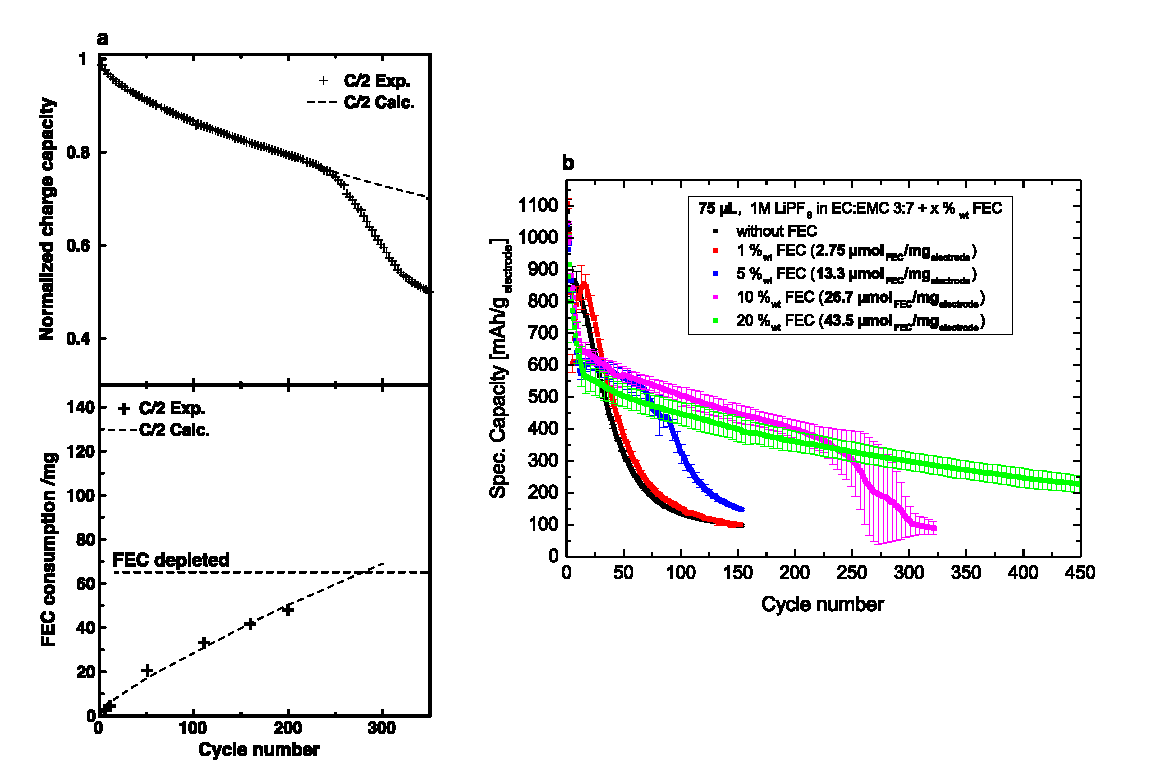
\includegraphics[scale=0.9]{figures/fec_depletion.eps}
}
Adapted from Figure 8 of Petibon et al.\cite{petibon_studies_2016} and Figure 1 of Jung et al.\cite{jung_consumption_2016}

This knee pathway has a number of interesting implications.
First, since laboratory-built cells are often filled with high electrolyte volumes, knee mechanisms that are not present in lab testing may manifest in more commercially representative form factors.
As Wetjen et al.\cite{wetjen_differentiating_2017} emphasize,
maintaining representative electrolyte volumes in lab-scale cells is critical for accurately capturing this knee pathway in production-scale cells.
Second, nominally identical cells, cycled identically, but with different initial FEC concentrations exhibited minute electrochemical differences before the knee.\cite{jung_consumption_2016}
Theoretically, only the FEC consumed in a given cycle manifests in the electrochemical signals from cycling (e.g., differential capacity or differnetial voltage analysis); the excess FEC is not electrochemically detectable as it does not participate in reactions with the electrode.
Since the \emph{remaining} FEC amount is the main determinant of cycle life in these cells, the knee point of cells exhibiting this mechanism is not predictable via standard electrochemical signals.
An interesting proposal for future work is to evaluate other nondestructive probes (e.g., electrochemical impedance spectroscopy\cite{zhang_identifying_2020}, acoustic signals\cite{knehr_understanding_2018}) that may be sensitive to FEC concentration in the electrolyte.

\subsection{Electrode connectivity}

Electrolyte dry out OR electronic connectivity
(From Tino, Peter can write) Kupper et al.~\cite{kupper_end--life_2018} model what they call `sudden death' by introducing a percolation threshold in the activity-saturation relationship, which is linked to electrolyte dry-out. This percolation behavior of the liquid electrolyte is similar, but not identical, to the one studied for ``effective diffusive conductivity`` and tortuosity by Ferguson and Bazant (Edwin: We can re-use (after asking for permission) Fig. 5 in Kupper's paper and Fig. 10 in Ferguson's paper here to illustrate the percolation threshold.)

Electronic connectivity: Li, Meyer et al

Distinct from LAM causing plating, as this can cause a knee in its own right

No experimental validation, but plausible

Create figure

\subsection{Mechanical degradation}
In addition to pressure plating, and percolation 
Figure with mechanical degradation knees
\paragraph{Pressure.}
pressure can be set and measured with pouch \cite{wunsch_investigation_2019} and prismatic cells\cite{cannarella_stress_2014} ,only measured on cylindrical \cite{willenberg_high-precision_2020}

High stack pressure can cause knee. High mechanical stress is not evenly distributed throughout the inside of the pouch, causing heterogeneous delamination, surface film formation, and uneven lithium distribution. LAM attributed to anode from half-cell data, no change in LAM PE. There's a sweet spot for stack pressure, just like temperature.\cite{cannarella_stress_2014}

Pressure evolution different for different kinds of bracing (Wünsch et al.) Thickness increase for unbraced cells correlated with knee point. Lifetime can be increased from 500 to 3200 cycles with the right bracing. (Wünsch et al.)

CT study on 18650s reveals jelly roll deformation, pfang et al. \cite{pfrang_long-term_2018} using cells from Ecker et al. \cite{ecker_calendar_2014}
Pressure can enhance conductivity and particle link, and heterogenous pressure induces uneven ageing for example due to ageing \cite{bach_nonlinear_2016}

The effects discussed here are inherently multidimensional (at the macroscale) in nature and hence cannot be captured by standard electrochemical models, which are one-dimensional at the macroscale. Instead, they would require complex three-dimensional models, whose computational complexity is prohibitively high for simulating degradation over hundreds of cycles. We are not aware of any current modeling efforts in this direction [right?]. One reduced-order modeling approach could be to couple one-dimensional electrochemical models with network models for the jellyroll [cite Tranter].

\paragraph{Interaction of SEI growth with mechanical effects.} [NEED TO CHECK HOW THIS IS DIFFERENT TO THE LAM SECTION IN PLATING]
Another possible mechanism that leads to a kneepoint is the accelerating SEI growth due to mechanical effects (stress and/or loss of active material).

This can occur, and be simulated, in various forms.
Laresgoiti et al.~\cite{laresgoiti_modeling_2015} introduce a fatigue model for loss of active material due to stress. They further show that particle volume changes lead to cracking of the SEI, which then exposes fresh particle surface causing accelerated SEI formation. Kupper et al.~\cite{kupper_end--life_2018} include this effect in a degradation model by directly including an empirical dependence on the tangential stress on the SEI layer into the SEI reaction term. In fact, as shown by Reniers et al.~\cite{reniers_review_2019}, even coupling Laresgoiti's model with a stress model (ignoring SEI growth) would lead to an accelerating growth rate since there is a positive feedback loop between higher stress and higher loss of active material.

A significantly different mechanism is proposed by Lin et al.~\cite{lin_comprehensive_2013}, who propose a mechanism whereby a combination of loss of lithium inventory (due to SEI reaction) and loss of active material in the positive electrode (due to Manganese dissolution) lead to a shift in the stoichiometry windows, which eventually accelerates the SEI reaction causing a knee point.
Jana et al.~\cite{jana_physical_2019} also include both SEI formation and loss of active material in their model, and have knee point effects that they attribute to `mechanical effects', but do not propose a model for how LAM contributes to these mechanical effects and instead leave them as `unmodeled'.
Check Dubarry's Cn/Cp mechanism.
Check Keil.

Rainflow model for stress in batteries: Xinran Xiao (Michigan State), Deshpande battery fatigue

Nice figures for this in Kupper 2018, Louli 2019.

\paragraph{Mechanics leading to plating}
Clamping pressure by hose clamp Bach et al. \cite{bach_nonlinear_2016}
Pressure with ball Fuchs et al. \cite{fuchs_post-mortem_2019}
Unusual forms and pressure Liu et al. 2018 \cite{liu_size_2018}
Seperator clogging Liu et al. 2020 \cite{liu_effects_2020}

\section{Other considerations}

We surveyed the literature to identify empirical case studies in which the knee point can be controlled via changes to a single variable. Table S1 classifies these case studies into three categories based on the nature of the variable: design, testing conditions, and sampling variability (a special case of these two categories). Some testing conditions have an obvious impact on the emergence of the knee. For example, higher charging rates and wider cycling voltage ranges accelerate the appearance of the knee. However, the impact of other variables is less clear. 

Yuliya: Maybe the way to frame this section is: some variables have a consistent impact whereas the impact of other variables is situation-specific.

\subsection{Ambiguous experimental effects}

\subsubsection{Discharging rate}

Unlike charging rate, the effect of discharging rate on the knee point is mixed.

Keil et al.\cite{keil_charging_2016} illustrated how discharging current had no effect on LMO+NMC/graphite and LCO+NCM/graphite cylindrical cells, but a lower discharging current (3A, 2.7C) lead to faster degradation than a higher discharging current (5A, 4.5C) for an LFP/graphite cylindrical cell when charged at 4.5C; they did not identify a mechanism. 
Similarly, Keil et al.\cite{keil_linear_2019} found that increasing discharging current from 1C to 2C lead to the elimination of the knee in graphite/NMC cylidrical cells.

Atalay et al.\cite{atalay_theory_2020} found that reducing the discharge rate from 4C to 1C accelerated the knee for 18650 NCA/Gr cells.
Omar et al. \cite{omar_lithium_2014} found that a higher discharging rate (1C to 15C) accelerated the knee for cylindrical LFP/Gr cells.

Diao et al.\cite{diao_accelerated_2019} showed no effect of discharge rate except at 60°C, where the cells discharged at 2C degraded almost twice as quickly than the cells discharged at 0.7C or 1C. 

Discharging can lead to worse cycle life due to higher temperature; other mechanisms? Most of the studies have found little impact or that slower discharge rate is worse. This may be a calendar aging effect? Faster discharge = less time spent cycling = less calendar aging. 

\subsubsection{Rests}

The effect of rests during cycling is unclear.

Keil et al.\cite{keil_linear_2019} found that decreasing rest time at both TOC and BOD from 900s to 10s delayed the knee point in graphite/NMC cylidrical cells.

Ma et al.\cite{ma_editors_2019} found an identical result: removing the 30 min rests at both TOC and BOD delayed the knee, but only with an upper cutoff voltage of 4.3 V. No effect at 4.1 V.

Rationalized by less time at high potential when plotted as a function of cycle number

In contrast, Epding et al.\cite{epding_investigation_2019} found that longer rest times in between rounds of cycling helped. This rest offered reversibly plated Li time to reintercalate.

\subsection{Sampling variability}

Nominally identical cells cycled identically often show differences in knee behavior. This sampling variability includes both intrinsic variability from manufacturing (component-level variation, cell assembly, etc) and extrinsic variability from testing (cycler calibration, temperature control, etc). These sources of variability cannot be distinguished.

The magnitude of sampling variability is a function of the cell design, manufacturing variability, and testing conditions. Sampling variability may increase with more aggressive cell designs, more manual cell assembly processes, and more aggressive testing conditions (particularly for test setups with no or poor temperature control). The magnitude of sampling variability can be estimated using studies with fairly large sample sizes (i.e., at least ~10 cells). Baumhöfer et al.\cite{baumhofer_production_2014} examined such variation in 48 cells and Harris et al.\cite{harris_failure_2017} in 24 cells. Note that these studies did not identify a correlation between cells...

\section{Conclusions and future work}

\section{Supporting Information}

 


Table S1. Summary of experimental variables leading to knee points


Yuliya: See table in Excel document tab 'SI-Exp Tables'. 


Table S2 classifies previous efforts to model the knee point as physics-based, equivalent circuit, or empirical. [add explanation of table columns]

Table S2. Summary of previous knee point modeling efforts

\bibliographystyle{myIEEEtran}
\bibliography{refs_zotero}




\end{document}
